\def\theTopic{ Music for Studying }
\def\dayNum{10}


\begin{center}
\vspace*{.1in}
{\bf {\large Does Music Help Us Study?}}\\
\end{center}
\vspace{-.1in}


Suppose you have a big test tomorrow and need to spend several hours
tonight preparing.  You'll be reviewing class notes, rereading  parts
of the textbook, going over old homework -- you know the drill.
\begin{enumerate}
\item  Which works better for you: turn on music, or study in silence? 
  Circle one:
  \begin{alist}
    \item With music
    \item In silence
  \end{alist}
  %Share answers with your group.  
  If you like to study with music (at least some times) describe:
  \begin{enumerate}
  \item what volume?\\
  \item with lyrics? or instrumental?\\
  \item what general category do you prefer?\\
  \end{enumerate}
% \item Does your group all agree?   (We doubt that.)  Do you use music
%   differently depending on the task?  Explain three or four factors
%   which influence your decision to pick a type of (or no) music.
% \begin{students}
%         \vspace{4cm}
% \end{students}
% \begin{key}
%   \\ {\it We hope that they list characteristics like
%     lyrics/instrumental, tempo, genre, mood of music.}
% \end{key}

\item A researcher wants to know if some types of music  improve or
  hurt the effectiveness of studying.  Suppose we want to address
  this question by getting college students to fill out a survey.
  \begin{enumerate}
  \item \label{response1} The survey will ask for details on the music
    type each student
    prefers for studying, but we will also need a way to measure how
    effective their studying is.  How could we measure a {\bf
      response} to use for comparison --  to see how much people are
    learning while studying?
\begin{students}
        \vspace{3cm}
\end{students}
\begin{key}
  \\ {\it This is tough. We want them to wrestle with questions of how
  much subjects knew before studying, how good a student they are, etc.
  (more in next question).  Good responses:  a post-test
  minus pre-test difference or we pick a topic which
  people don't generally know about before they study.}
\end{key}
     \item\label{lurking} In discussing the response, you probably
       found difficulties which make it hard to compare people.  What
       differences in students 
       make it hard to get a clear comparison between different music
       types?  List at least three variables that we should consider.
       For each: is it categorical or quantitative?  Focus in on
       one categorical and one quantitative variable.
\begin{students}
        \vspace{5cm}
\end{students}
\begin{key}
  \\ {\it Some students are just smarter than others (IQ is
    quantitative). The subject area of the test they are studying for (anatomy
    versus philosophy?) -- categorical. Years of musical training
    (quantitative). Surroundings (dorm room versus library) -
    categorical. Age (quantitative.) }
\end{key}
  \end{enumerate}
\item Another option for studying the effect of music type on studying is
  to {\bf assign treatments}, as in this study from 2014.  \\
   Perham, N. and Currie, H (2014). Does listening to preferred music
   improve reading comprehension performance? {\em Applied Cognitive
     Psychology} {\bf 28}:279--284.

  
   They used four levels of the variable \verb|sound|: ``disliked
   lyrical music (DLYR), liked lyrical music (LLYR), non--lyrical
   music (NLYR) and quiet (Q)'' and each subject chose music they
   liked with lyrics (LLYR), while the instrumental music (NLYR) was
   picked by the researchers, and subjects were screened to be sure they
   did not enjoy ``thrash'' music, which was used for DLYR.  Subjects
   were told to ignore the music, and had to read 70 lines of text,
   then answer four multiple choice questions about the reading (taken
   from SAT exams). They repeated the task for three more readings
   (with 4 questions each), and the proportion correct was recorded.

  \begin{enumerate}
    \item  Is use of the SAT questions an improvement over your choice
      of response in \ref{response1}?  Explain why or why not.
\begin{students}
        \vspace{4cm}
\end{students}
\begin{key}
  \\ {\it SAT will generally be better because it allows us to use a
    comparable measure across all subjects, and it is immediately
    following the music treatment.}
\end{key}
   \item   Is use of the four \verb|sound| treatments an improvement
     over asking students how they study?  Explain why or why not.
\begin{students}
        \vspace{4cm}
\end{students}
\begin{key}
  \\ {\it The four treatment levels are generally be better because
    they take away many of the options people have when choosing music.
      We can then get a direct comparison of music versus no music and
      of lyrical versus instrumental music.}
\end{key}
  
  \end{enumerate}

\item In an {\bf experiment} levels of the explanatory (treatment)
  variable are {\bf assigned} to subjects (or units if people are not
  involved). In order to allow statistical inference, we should assign the
  treatments at random, making it a {\bf randomized experiment}. 
  In an {\bf observational study} we simply record levels or values of
  the explanatory variable instead of assigning them.  Looking back at
  the studies above, which was an experiment?
\begin{students}
        \vspace{1cm}\\
\end{students}
\begin{key}
  \\ {\it  The second one from the article by Perham and Currie.}\\
\end{key}
  Which was an observational study?  Explain how you know this.
\begin{students}
        \vspace{1cm}\\
\end{students}
\begin{key}
  \\ {\it  The survey would be observational, because music levels are
    not assigned.}
\end{key}

\end{enumerate}


\begin{center}
  {\bf Advantages of Randomized Experiments}
\end{center}

To make sure we're all thinking of the same response for our study on
the effect of music while studying, we'll focus on using the SAT
reading comprehension scores as our response.  Music (or quiet) will
be played while our subjects read and answer the questions.

\begin{enumerate}
  \setcounter{enumi}{5}
  \item In \ref{lurking}, above you mentioned several attributes of
    people which would indicate who does better on a test.  One such
    variable would be IQ.  Smarter people tend to get higher scores on
    the SAT.  
    \\ We refer to a variable like IQ as a {\bf lurking} variable when
    we do not measure it and take it into account.  What other lurking
    variables did you identify in \ref{lurking} (or add some here to
    get at least three)
    which would cause some people to do better on SAT than others?
\begin{students}
        \vspace{1cm}\\
\end{students}
\begin{key}
  \\ {\it  AWV}
\end{key}
  \item  If we don't measure IQ and don't adjust for it, we won't be
    able to tell whether one group did better because it had higher
    mean IQ, or because they were assigned the more effective treatment.  
    Let's see what happens to mean IQ (and another variable - SAT
    prep) if we randomly separate 12
    people into treatment (music) and  control (quiet) groups of 6 each.

    
\begin{tabular}{|r|c|c||r|c|c|}\hline
      \multicolumn{3}{|c||}{Treatment} &\multicolumn{3}{|c|}{Control}\\
  Name  & IQ & SAT prep & Name & IQ &SAT prep \\
\hline
Andy & 104 & Y &Peter &106 &Y\\
\hline
Ben  & 118 & Y & Maria & 90 &N\\
\hline
Betty & 79 & N & Marti & 97 &N \\
\hline
Jorge & 94 & Y & Mikaela& 98 &N\\
\hline
 Kate  & 106&N &  Patty &89 &N\\
\hline
Russ  &  88 &Y & Shawn &85 &Y\\ \hline
\end{tabular} \hfill
\begin{minipage}{.40\linewidth}
  Mean IQ of treatment group: 98.2

  Mean IQ of control group: 93.8

  Difference in means:  4.4
\end{minipage}

Write Name, IQ, and whether or not they took an SAT prep class (Yes or
No) for each person on an index card.
(If the cards are already started, check that you have the right
names and values.)  
   \begin{enumerate}
   \item Mix the cards thoroughly, and deal them into two piles of six
     each, labeling one ``T'' and the other ``C''.
     Compute the mean IQ for each group and take the difference
     ($T - C)$.\vspace{1cm}
   \item Plot your difference as instructed by your teacher. \vspace{1cm} 
\end{enumerate}

\item As with many techniques in statistics, we want to see what
  happens when we repeat the process many times.  Doing this by hand
  many times gets tedious, so we will use the computer to shuffle and
  compute means for us. \\ Go to:
  \url{http://shiny.math.montana.edu/jimrc/IntroStatShinyApps} and click
  ``Enter Data'' under \underline{One of each}. \\
   Select \fbox{Use PreLoaded Data} and \fbox{SATprep}.
 \begin{minipage}{.50\linewidth}
{\footnotesize
\begin{verbatim}
group iq
t 104
t 118
t 79
t 94
t 104
t 90
c 97
c 98
c 88
c 106
c 89
c 85
\end{verbatim}
}
 \end{minipage}
\begin{key}
  \begin{minipage}{.50\linewidth}
    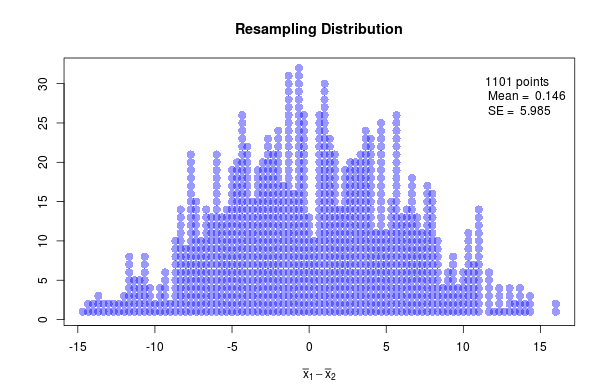
\includegraphics[width=\linewidth]{plots/IQ-shuffle.png}
  \end{minipage}
\end{key}

 Again under the \fbox{One of Each} menu, click \fbox{Test}
 Click \fbox{\sf 1000} several times.   Record
the difference in means for the first shuffle.\\

\item As we said above, we need to think about repeating the shuffling
  process over and over.  Click \fbox{5000} and sketch the
  right-hand plot (above).  Describe the center,
  spread, and shape of this distribution.
  \begin{list}{}{}
  \item[center]
\begin{students}
 \ \  \\
\end{students}
\begin{key}
  {\it  Near 0 (0.033). Why are mine always positive?  }
\end{key}
  \item [shape]\ 
\begin{students}
 \ \  \\
\end{students}
\begin{key}
  {\it  Symmetric  }
\end{key}
  \item [spread]\
\begin{students}
 \ \  \vspace{2cm}
\end{students}
\begin{key}
  {\it  around 6}
\end{key}
  \end{list}

\item Do we get the same pattern in the right hand plot if we run
  another batch of shuffles, say 10,000 this time?    Do
  center, shape, and/or spread change?
\begin{students}
        \vspace{2cm}\\
\end{students}
\begin{key}
  \\ {\it  No, all remain about the same.}
\end{key}


\item  Does randomization always make mean IQs the same
  between the two treatment groups? Explain. 
\begin{students}
 \vspace{3cm} 
\end{students}

\begin{key}
  {\it  Not exactly in every single trial though on average (over many
    shuffles) the groups are   equivalent.  }
\end{key}
  
\item  Does randomization tend to balance out mean IQ in the long
  run, after many trials? Explain. 
\begin{students}
 \vspace{3cm} 
\end{students}

\begin{key}
  {\it  Yes because the distribution of the difference between the two
   group means is centered at 0. }
\end{key}


  
\item {\bf Very Important Question:}  In general, how similar are
  group mean IQs when we randomly assign people into two groups?
\begin{students}
        \vspace{4cm}\\
\end{students}
\begin{key}
  \\ {\it  The difference in mean IQ between two randomized groups
    will be close to zero most of the time.  There is no guarantee for
  any one sample, but in general randomization makes the groups very
  similar.} 
\end{key}

% \item If we randomly assign levels of sound -- for simplicity, just
% LLYR or Q -- to subjects, and then find that the Q group had a much
% higher mean score on the SAT questions than the LLYR group, might 

\item Another lurking variable would be the fact that some people have
  taken a short course as an SAT prep and others haven't.  If the
  course does what it claims, then it could be the reason for one
  group to score higher than the other. We will look at the
  proportions who have taken an SAT prep course in the treatment and
  control groups.  
  \begin{enumerate}
  \item Is ``took SAT prep course'' a categorical or quantitative
    variable? 
\begin{students}
        \vspace{1cm}\\
\end{students}
\begin{key}
  \\ {\it categorical}
\end{key}
    \item Again go to the  web app and click ``Enter Data'' under
      \underline{Two Categ.}  Suppose 
      we are randomly assigning 100 people to our two groups, and that
      28 of them have taken SAT prep, 72 have not. Put in 14 Successes
      for each group, and 36 Failures for each.  Click \fbox{\sf Use
        These Data} and make sure that we have 50 in each group (1 =
      treatment, 2 = control), 28 ``Successes'' (took SAT prep) and 72
      ``Failures''. (This is just one way to get the right totals at
      the edges, or margins, of the table.  Because we'll be doing
      lots of shuffles, the groups do not have to start out as balanced,
      but it makes it easy to get the right marginal totals.) Click 
      ``Test''\\
fixme:\\
      and  click \fbox{\sf Shuffle}.  (Leave the Cards option checked)\\
      What totals do you get for blue and green cards?  What do the
      colors represent?
\begin{students}
        \vspace{1cm}\\
\end{students}
\begin{key}
  \\ {\it 28 blue, 72 green. Blue = success  = SAT prep, green =
    ``Failure'' or no SAT prep.}
\end{key}
       \item For this shuffle, what is the difference in proportions? 
         Click \fbox{\sf Shuffle} four more times, and record all 5
         differences. 
\begin{students}
        \vspace{1cm}\\
\end{students}
\begin{key}
  \\ {\it AWV}
\end{key}
       \item Change number of shuffles to \fbox{\sf 5000} and click
         \fbox{\sf Shuffle}. Sketch your plot here.
\begin{students}
        \vspace{4cm}\\
\end{students}
\begin{key}
  
   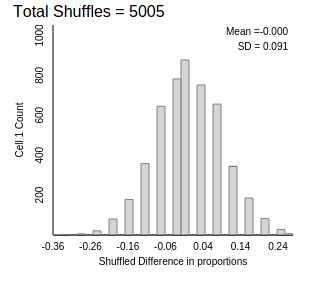
\includegraphics[width=.4\linewidth]{plots/SATprep-shuffles.png}
\end{key}
     \item Compare with other groups.  Do the pictures look the
       same?
\begin{key}
  {\it  Yes. }
\end{key}

  \begin{list}{}{}
  \item[center]
\begin{students}
 \ \  \\
\end{students}
\begin{key}
  {\it  Near 0 (0.00).   }
\end{key}
  \item [shape]\ 
\begin{students}
 \ \  \\
\end{students}
\begin{key}
  {\it  Symmetric  }
\end{key}
  \item [spread]\
\begin{students}
 \ \  \vspace{2cm}
\end{students}
\begin{key}
  {\it  around 0.09}
\end{key}
  \end{list}

\end{enumerate}

\item When we randomly assign people to two groups:
  \begin{enumerate}
  \item Is it possible for a categorical lurking variable like SAT prep
    to be imbalanced across the two groups?  Explain.
\begin{students}
    \vspace{1.5cm}\\
\end{students}
\begin{key}
  \\ {\it Yes, the proportions might differ by as much as 0.25.} 
\end{key}
  \item Will the lurking SAT variable ``usually'' be poorly balanced
    across the two groups?  Explain.
\begin{students}
        \vspace{1.5cm}\\
\end{students}
\begin{key}
  \\ {\it  No. For most of the randomizations, we get a difference in
    proportion which is close to zero, which says that about the same
    proportion of treatment people as control people have taken SAT prep. } 
\end{key}
  \end{enumerate}

\item In general, how similar is the proportion of people who have
  taken SAT prep in the treatment group to the same proportion in the
  control group? 
\begin{students}
        \vspace{3cm}\\
\end{students}
\begin{key}
  \\ {\it  The difference in proportion with SAT prep between two
    randomized groups will be close to zero most of the time.  There
    is no guarantee for any one sample, but in general randomization
    makes the groups very similar.} 
\end{key}
\item If you ran an experiment where you randomly assigned people to
  either listen to music or silence, would you have to worry about the effect
  of SAT prep courses on the results?  Explain. 
\begin{students}
        \vspace{6cm}\\
\end{students}
\begin{key}
  \\ {\it We can be pretty sure that the two randomized groups have
    similar proportions of people in them who took the SAT prep.
    Therefore, it's not a problem, and we can make out conclusions on
    the effects of music without worry about lurking variables.}
\end{key} 
\end{enumerate}





\begin{center}
  {\bf Take Home Messages}
\end{center}
  \begin{itemize}
  \item Vocabulary:  response variable, explanatory variable,
    experiment, randomized experiment, observational study, lurking
    variable.
  \item This lesson is critical for understanding how experiments
    differ from observational studies.  When we assign treatments at
    random, we ``even out'' any lurking variables, so we can say that
    differences we observe are caused by the explanatory variable (the
    treatment). We call this {\bf causal inference}.
  \item  Our use of the web app today was to see what happens to means
    of a lurking variable when we randomly split people into two
    groups. You should have concluded that the means tend to be
    approximately equal (difference in means is centered at zero), and
    that the distribution of the difference in means is symmetric. Any
    positive value has a negative counterpart which just involves
    swapping the labels (T $\longleftrightarrow$ C).\\
   We will use these apps later to evaluate treatment effects, but
   today we are only looking at  lurking   variables. 
 \item 
  Use the remaining space for any questions or your own summary of the
  lesson. 
  \end{itemize}
  



 % means <- c(.38, .54, .37, .61)
 % sds <- c(.04, .05, .04, .05)
 % sound <- c("DLYR","noLYR","LLYR","Quiet")
 % (.61-.54)/sqrt(2*.05^2/8)
 % trt iqs
 %  t 104
 %  t 118
 %  t  79
 %  t  94
 %  t 104
 %  t  90
 %  c  97
 %  c  98
 %  c  88
 %  c 106
 %  c  89
 %  c  85
